\documentclass[]{book}
\usepackage{lmodern}
\usepackage{amssymb,amsmath}
\usepackage{ifxetex,ifluatex}
\usepackage{fixltx2e} % provides \textsubscript
\ifnum 0\ifxetex 1\fi\ifluatex 1\fi=0 % if pdftex
  \usepackage[T1]{fontenc}
  \usepackage[utf8]{inputenc}
\else % if luatex or xelatex
  \ifxetex
    \usepackage{mathspec}
  \else
    \usepackage{fontspec}
  \fi
  \defaultfontfeatures{Ligatures=TeX,Scale=MatchLowercase}
\fi
% use upquote if available, for straight quotes in verbatim environments
\IfFileExists{upquote.sty}{\usepackage{upquote}}{}
% use microtype if available
\IfFileExists{microtype.sty}{%
\usepackage{microtype}
\UseMicrotypeSet[protrusion]{basicmath} % disable protrusion for tt fonts
}{}
\usepackage{hyperref}
\hypersetup{unicode=true,
            pdftitle={Embrace the Serpent: A Neuroscientific Perspective on Archetypes},
            pdfauthor={Dr.~Dominique Makowski},
            pdfborder={0 0 0},
            breaklinks=true}
\urlstyle{same}  % don't use monospace font for urls
\usepackage{natbib}
\bibliographystyle{apalike}
\usepackage{longtable,booktabs}
\usepackage{graphicx,grffile}
\makeatletter
\def\maxwidth{\ifdim\Gin@nat@width>\linewidth\linewidth\else\Gin@nat@width\fi}
\def\maxheight{\ifdim\Gin@nat@height>\textheight\textheight\else\Gin@nat@height\fi}
\makeatother
% Scale images if necessary, so that they will not overflow the page
% margins by default, and it is still possible to overwrite the defaults
% using explicit options in \includegraphics[width, height, ...]{}
\setkeys{Gin}{width=\maxwidth,height=\maxheight,keepaspectratio}
\IfFileExists{parskip.sty}{%
\usepackage{parskip}
}{% else
\setlength{\parindent}{0pt}
\setlength{\parskip}{6pt plus 2pt minus 1pt}
}
\setlength{\emergencystretch}{3em}  % prevent overfull lines
\providecommand{\tightlist}{%
  \setlength{\itemsep}{0pt}\setlength{\parskip}{0pt}}
\setcounter{secnumdepth}{5}
% Redefines (sub)paragraphs to behave more like sections
\ifx\paragraph\undefined\else
\let\oldparagraph\paragraph
\renewcommand{\paragraph}[1]{\oldparagraph{#1}\mbox{}}
\fi
\ifx\subparagraph\undefined\else
\let\oldsubparagraph\subparagraph
\renewcommand{\subparagraph}[1]{\oldsubparagraph{#1}\mbox{}}
\fi

%%% Use protect on footnotes to avoid problems with footnotes in titles
\let\rmarkdownfootnote\footnote%
\def\footnote{\protect\rmarkdownfootnote}

%%% Change title format to be more compact
\usepackage{titling}

% Create subtitle command for use in maketitle
\providecommand{\subtitle}[1]{
  \posttitle{
    \begin{center}\large#1\end{center}
    }
}

\setlength{\droptitle}{-2em}

  \title{Embrace the Serpent: A Neuroscientific Perspective on Archetypes}
    \pretitle{\vspace{\droptitle}\centering\huge}
  \posttitle{\par}
    \author{Dr.~Dominique Makowski}
    \preauthor{\centering\large\emph}
  \postauthor{\par}
      \predate{\centering\large\emph}
  \postdate{\par}
    \date{2019-11-02}

\usepackage{booktabs}
\usepackage{amsthm}
\makeatletter
\def\thm@space@setup{%
  \thm@preskip=8pt plus 2pt minus 4pt
  \thm@postskip=\thm@preskip
}
\makeatother

\begin{document}
\maketitle

{
\setcounter{tocdepth}{1}
\tableofcontents
}
\hypertarget{introduction}{%
\chapter{Introduction}\label{introduction}}

\begin{center}\rule{0.5\linewidth}{\linethickness}\end{center}

\textbf{Disclaimer: This is a compilation of thoughts that might be someday used in a fictional novel. It does not reflect any personal beliefs.}

\textbf{Warning: This is a work in progress, i.e., currently just a collection of unstructured information.}

\begin{center}\rule{0.5\linewidth}{\linethickness}\end{center}

The idea that the mind is deeply structured along universal lines has always been fascinating to me. Although strongly criticized and mostly debunked by science, the idea that the mind was structurally clustered in a similar way across the time and space has endured, quitting the prison of scientific psychology to pervade other fields, such as history of arts, literature and anthropology. In fact, the notion of archetypes and archetypal patterns has become quite popular, evidence being ``found'' within the redundancies of Human behaviours, myths and stories of old.

\textbf{But beyond the scent of pseudoscience that emanates from this concept, do archetypes make any scientific sense?}

Archetypes as they are commonly defined and conceptualized are hardly compatible with the current scientific knowledge. For instance, Jung's collective unconscious has no place in light of what we know about neurogenesis, neurodevelopment and functional and structural neuroanatomy. Similarly, research on personality does not support the existence of clusters, or profiles, that would resemble commonly described archetypal figures (such as the warrior, the hero, the wise old man, etc.). Nonetheless, I think (and hope), that a scientific approach is possible and potentially interesting. Thus, the goal of this book is to provide a new and rational perspective on archetypes, informed by biology, psychology and neuroscience.

My own journey started as a naive interest for psychoanalysis in general, and a particular appeal for the deeply hidden core(s) of our being. But that fascination did not last. The first blow was given by the \emph{black book of psychoanalysis} \citep[``Le livre noir de la psychanalyse'';][]{borch2005livre}, that superbly and elegantly shattered most of the psychodynamic approach to pieces. \emph{Most of it} only, because Jung's ``Depth Psychology'' somehow resisted, keeping some level of appeal in the back of my mind. Possibly due to my shared interest for myths and history of religions, or to some other unconscious motivation, I found the Jungian mythological and cross-cultural perspective attractive (or at least interesting). But we need to face the serpent, and I could no longer ignore the evidence. And evidence is presented on a golden plate by \citet{lequellec2013jung}, in the excellent ``Jung et les archétypes. Un mythe contemporain'', casting doubt upon the whole Jungian enterprise. This second, finishing blow left me wondering; what is left of the archetypes in this landscape of burning ashes?

\textbf{As a phoenix, can this idea be reborn?}

\hypertarget{history-of-archetypes}{%
\chapter{History of Archetypes}\label{history-of-archetypes}}

\textbf{Warning: This is a work in progress, i.e., currently just a collection of unstructured information.}

\hypertarget{philosophical-roots}{%
\section{Philosophical roots}\label{philosophical-roots}}

It is common to mention Plato's Idea as the origin or philosophical basis for archetypes, mainly because of Carl Jung's supposed inspiration.

\hypertarget{carl-jung-1875---1961}{%
\section{Carl Jung (1875 - 1961)}\label{carl-jung-1875---1961}}

Jung is the one that gives to ``achetypes'' its \emph{modern} (in that sense) meaning in 1919. Originally named ``primordial images'' (a term he borrowed from the historian of art Jacob Burckhardt), Jung understood archetypes as universal, archaic patterns or images that derive from the collective unconscious, seen as the psychic counterpart of bodily instincts \citep{feist2009theories}. He makes a distinction between \emph{archetypes-as-such}, the underlying forms from which emerge motives that he refers to as \emph{archetypal images} (e.g., the mother, the child, \ldots). These archetypal images are made \emph{manifest} (i.e., explicit and consciously accessible) as they are filled with specific content through history, culture or personal history \citep{papadopoulos2012}.

In his later life, inspired by oriental philosophies, Jung used the term \emph{unus mundus} to describe the unitary reality which underlay all manifest phenomena. Jung expanded the notion of archetypes to the physical world itself, suggesting that ``psychoid'' archetypes (the non-psychic aspect of the archetype), fundamental principles of matter and energy, are the mediators of the unus mundus.

Critically, Jung's archetypes stem out of the \emph{collective unconscious}, therefore forming a substratum common to all humanity. The collective unconscious is, in Jung's perspective, referred to as the knowledge and experiences that we share as a species. A reminiscent echo of information passed down through generations from the dawn of mankind, and even afore.

Jung also named ``archetypes'' what could be seen as parts of the psyche. In particular, he focused on five of such dimensions:

\begin{itemize}
\tightlist
\item
  The \textbf{Anima} and the \textbf{Animus} are the feminine and masculine aspects of our Psyche. He mentions four distinct levels of development for the Anima, corresponding to its formation and evolution during the lifetime of an individual. \emph{Eve} is the first stage, where the anima emerges in the shape of the male's object of desire. She then becomes \emph{Helen} (of Troy, who sailed away from his husband), an independent and intelligent woman. She achieves virtue in \emph{Mary} (the purest figure in Christian tradition), and finally becomes \emph{Sophia}, the Greek goddess of wisdom.
\item
  The \textbf{shadow} is the part of one's Self to which the conscious ego does not identify.
\item
  The \textbf{Persona} refers to the image that a person presents to the world. According to Jung, the Persona is ``a kind of mask, designed on the one hand to make a definite impression upon others, and on the other to conceal the true nature of the individual''. It emerges from the amalgamation of what an individual wants to be, what he thinks he is, what other people think of him and what they want him to be.
\item
  The \textbf{Self} is the realised product of the integration of all conscious and unconscious aspects of our personality.
\end{itemize}

Interstingly, while the archetypal images (the manifest motives) are usually the main focus of interest, it is important to note that Jung himself warned against such simplification. Such ``definite mythological images of motifs {[}\ldots{]} are nothing more than conscious representations; it would be absurd to assume that such variable representations could be inherited''. Again, the true archetypes for Jung were their deeper, instinctual, fluid sources -- ``the `archaic remnants', which I call `archetypes' or `primordial images'\,'' \citep{jung1964approaching}.

Describe the excellent work by \citet{lequellec2013jung}.

\hypertarget{archetypal-interpretation-of-the-tarot}{%
\section{Archetypal Interpretation of the Tarot}\label{archetypal-interpretation-of-the-tarot}}

The first documented tarot packs were recorded between 1440 and 1450, and are likely to have entered Europe from Egypt in the late 14th century. The Tarot consists of 78 cards - 56 in the \emph{Minor Arcana} and 22 in the \emph{Major Arcana} (also known as the trump cards), which consists of the emblematic picture cards of a tarot deck. Although the tarot being a very old game, its interpretation as having a relationship with archetypes was kickstarted by Jung himself in \href{https://marykgreer.com/2008/03/31/carl-jung-and-tarot/}{1933}. ``They are psychological images, symbols with which one plays, as the unconscious seems to play with its contents.'' The content on these cards, said Jung, ``are sort of archetypal ideas, of a differentiated nature.''

\begin{figure}

{\centering 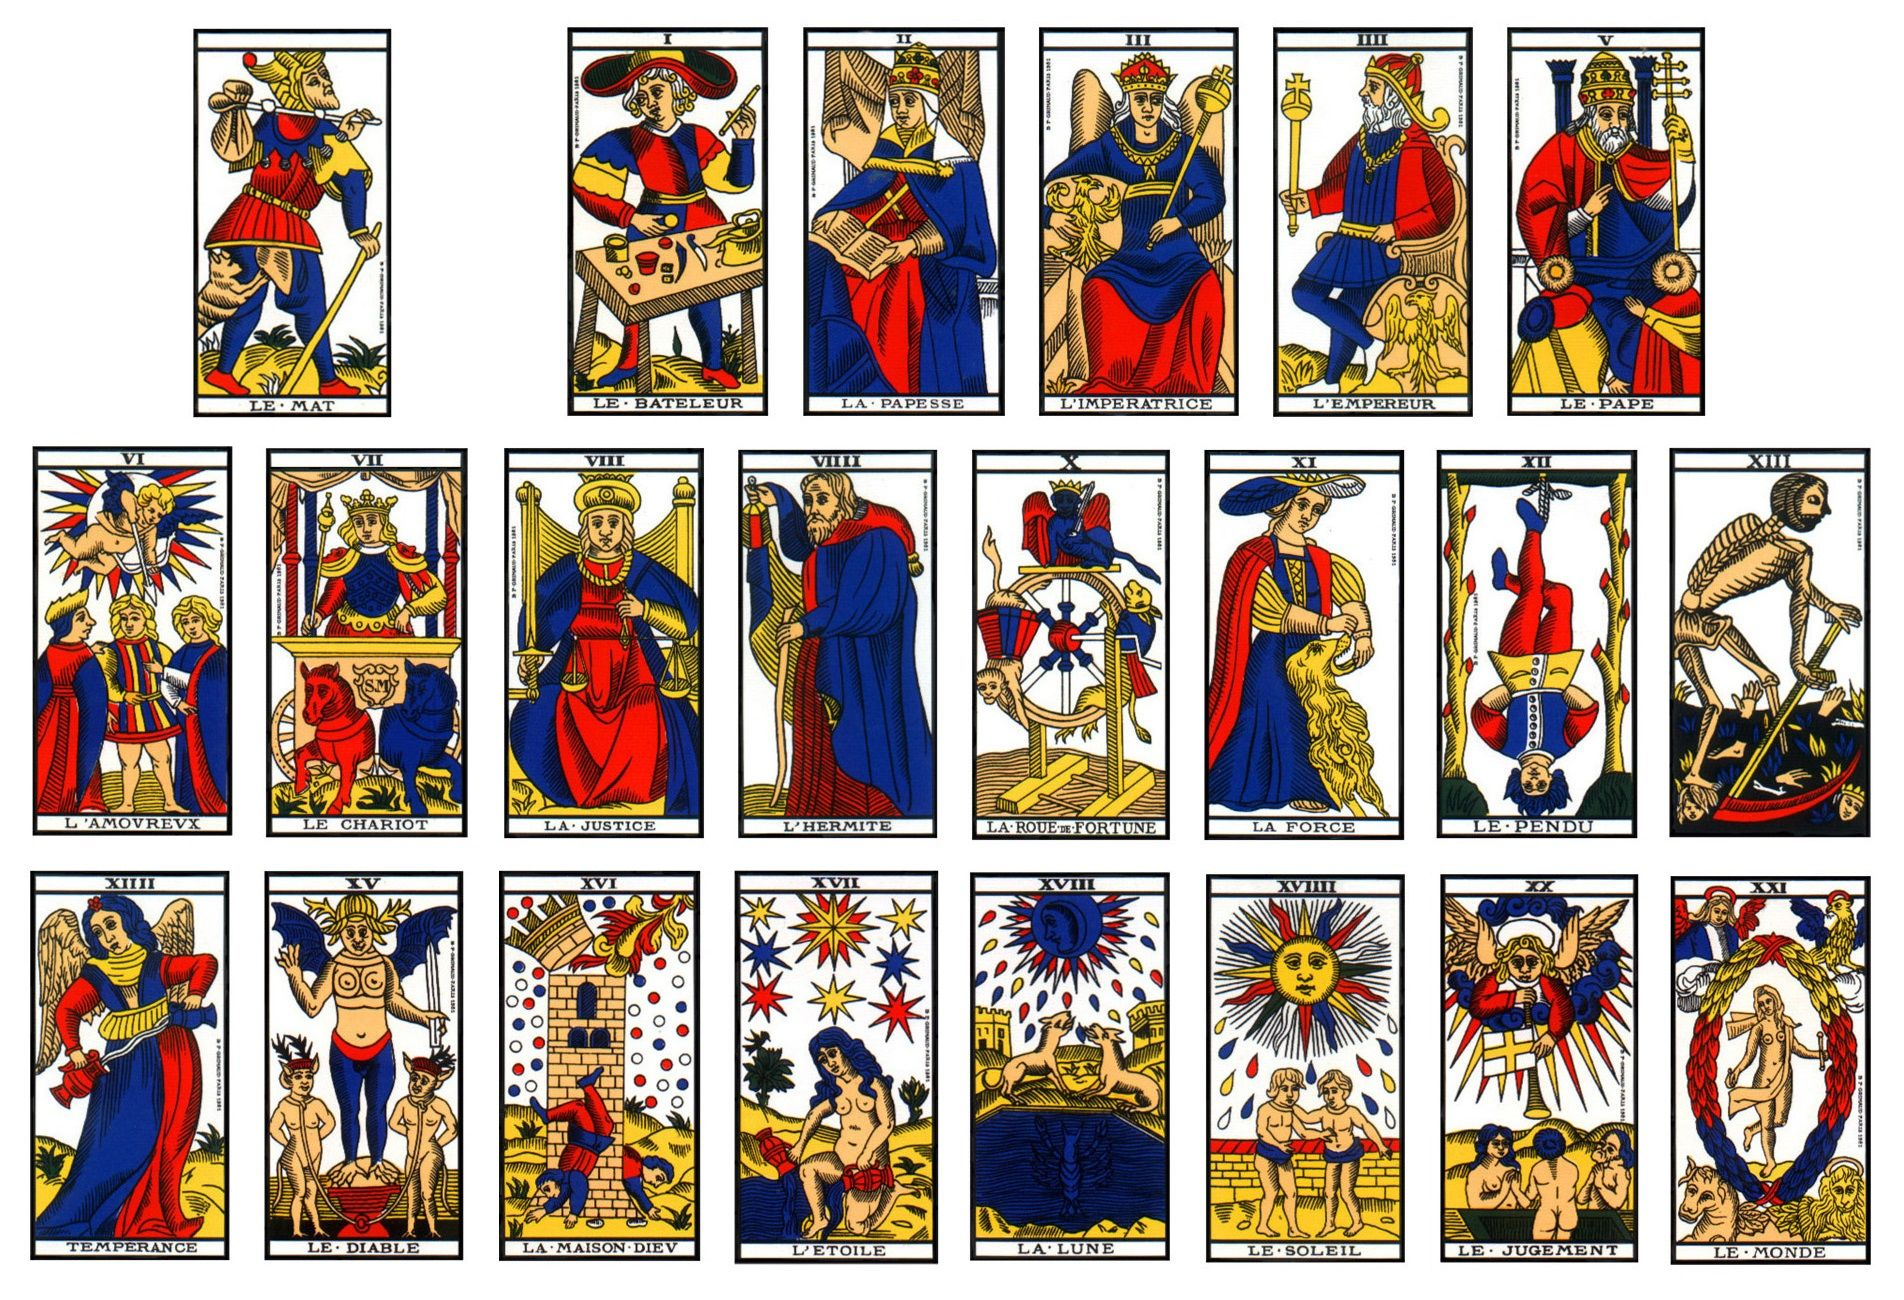
\includegraphics[width=\textwidth]{img/tarot} 

}

\caption{The 22 cards in the Major Arcana of the 'Tarot de Marseilles'.}\label{fig:unnamed-chunk-2}
\end{figure}

The \emph{Major Arcana} consists of 22 cards, numbered in Roman numerals from I to XXI, while The Fool is the only unnumbered card, sometimes placed at the beginning of the deck as 0, or at the end as XXII.

I. The Magician\textbackslash{}
II. The High Priestess\textbackslash{}
III. The Empress\textbackslash{}
IIII. The Emperor\textbackslash{}
V. The Hierophant\textbackslash{}
VI. The Lovers\textbackslash{}
VII. The Chariot\textbackslash{}
VIII. Strength\textbackslash{}
VIIII. The Hermit\textbackslash{}
X. Wheel of Fortune\textbackslash{}
XI. Justice\textbackslash{}
XII. The Hanged Man\textbackslash{}
XIII. Death\textbackslash{}
XIIII. Temperance\textbackslash{}
XV. The Devil\textbackslash{}
XVI. The Tower\textbackslash{}
XVII. The Star\textbackslash{}
XVIII. The Moon\textbackslash{}
XVIIII. The Sun\textbackslash{}
XX. Judgement\textbackslash{}
XXI. The World\textbackslash{}
XXII. The Fool\textbackslash{}

It is understandable that the mysterious origin of the Tarot, the esoteric figures, and critically the symbolic details present in them created a fertile terrain for all kinds of interpretations. Attempts to map these figures to Jungian concepts has been numerous. For instance, the Fool, representing carefree ignorance, has been connected with the unrealised Self. He carries a closed bag, said to contain the tools that could allow him to achieve wholeness. On the other side, the World card (XXI), representing completion nad success, was connected to the Self realised, as it shows an individual floating amongst the clouds. His nudity can be interpreted as transparency and revelation. What was hidden before has now become known. The four animals present in the corners corresponds to the four elements in Christian symbolism, and are interpreted as evidence that the individual has harnessed the four elements present within Nature (being the fifth element).

\hypertarget{joseph-campbell-1904---1987}{%
\section{Joseph Campbell (1904 - 1987)}\label{joseph-campbell-1904---1987}}

In ``The Hero with a Thousand Faces'', \citet{campbell1949hero}, inspired by Jung, presents his theory of the mythological structure of the journey of the archetypal hero extracted by comparing myths from different regions of the world. He identifies common tropes or characters, such as the young hero, the wise old man or woman, the shape-shifting woman or man, and the shadowy antagonist, that he relates to archetypes. He suggests that such myths and stories have a narrative structure that mirrors or echoes the psychological structure of the mind, which is the reason of their power.

\hypertarget{robert-moore-1942---2016}{%
\section{Robert Moore (1942 - 2016)}\label{robert-moore-1942---2016}}

In ``King Warrior Magician Lover'', \citet{moore1991king} discuss the four primary masculine archetypes:

\begin{itemize}
\tightlist
\item
  King
\item
  Warrior
\item
  Magician
\item
  Lover
\end{itemize}

To each one of these archetypes correspond an immature version:

\begin{itemize}
\tightlist
\item
  The Divine Child
\item
  The Hero
\item
  The Precocious Child
\item
  The Oedipal Child
\end{itemize}

In the same framework, feminine (altough not directly mentioned by the original authors) are:

\begin{itemize}
\tightlist
\item
  Queen
\item
  Mother
\item
  Wise woman
\item
  Lover
\end{itemize}

\hypertarget{carol-pearson-1944---present}{%
\section{Carol Pearson (1944 - Present)}\label{carol-pearson-1944---present}}

In ``The Hero and the Outlaw'', \citet{mark2001hero} discuss twelve archetypes:

\begin{itemize}
\tightlist
\item
  The Innocent
\item
  The Orphan / Everyman
\item
  The Hero
\item
  The Caregiver
\item
  The Explorer
\item
  The Rebel
\item
  The Lover
\item
  The Creator
\item
  The Jester
\item
  The Sage
\item
  The Magician
\item
  The Ruler
\end{itemize}

\begin{figure}

{\centering 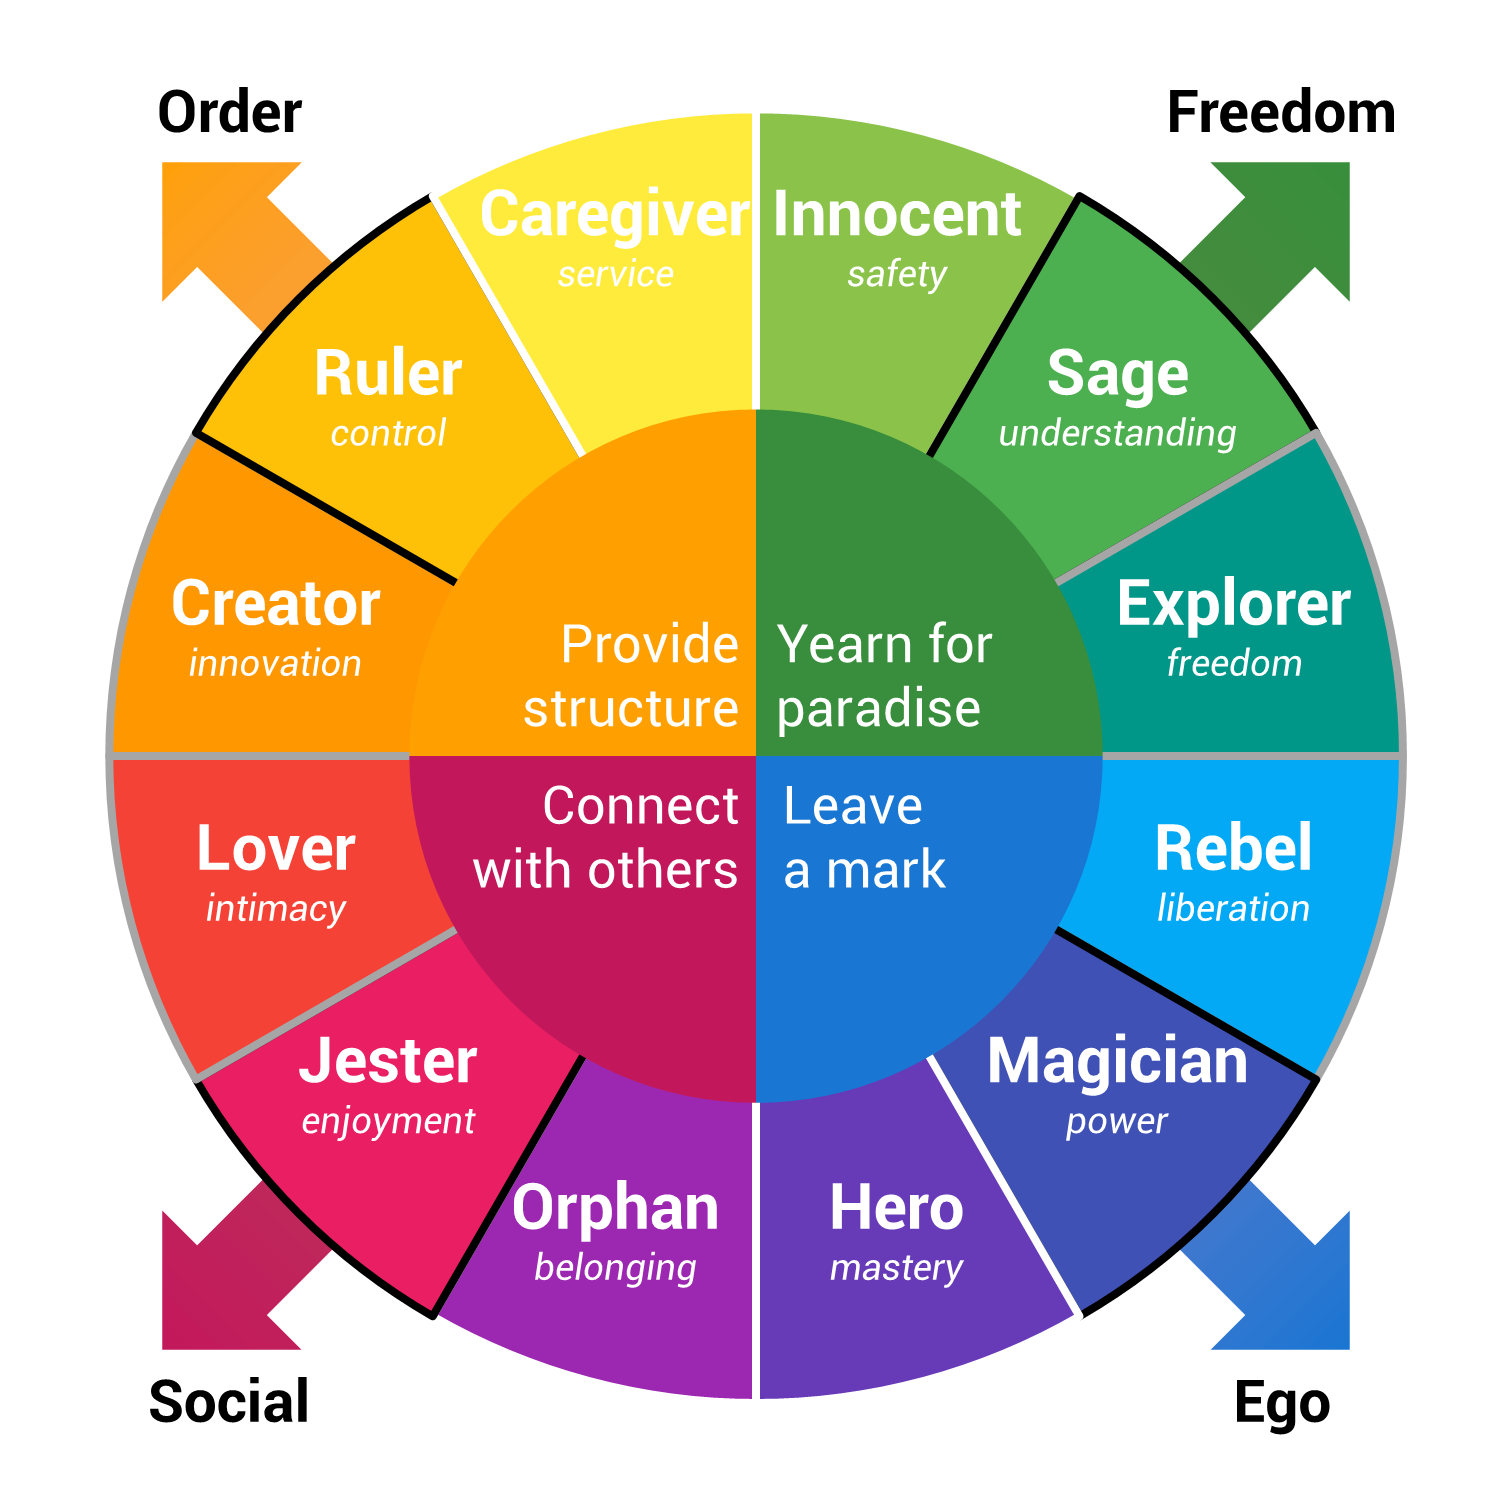
\includegraphics[width=\textwidth]{img/12archetypes} 

}

\caption{The 12 archetypes and the specific 'universal needs' that they address, grouped by their orientation (ego, order, freedom and social) and type (based on their 'driving source'): the diagonal archetypes (outline in black) correspond to the Self type, the vertical archetypes (outlined in white) to the Ego type, and the horizontal archetypes (outlined in grey) to the Soul type.}\label{fig:unnamed-chunk-3}
\end{figure}

This framework has been complexified, grouping these twelve archetypes into sets, for instance by classifying them into three types relative to their ``driving source''. For instance, the \emph{Ego} type (Innocent, Orphan, Hero and Caregiver) is driven to fulfill ego-defined agendas and \emph{mutatis mutandis} for the \emph{Soul} (Explorer, Rebel, Lover and Creator) and \emph{Self} (Jester, Sage, Magician and Ruler) types.

Additionally to the type, these archetypes can also be clustered according to their orientation on a two-dimensional plane with four cardinal points, which are \emph{Ego} (leaving a mark on the world), \emph{Order} (providing structure), \emph{Freedom} (yearning for paradise) and \emph{Social} (connecting to others), creating pairs of opposite (Social and Freedom being opposed to Ego Order, respectively).

The type and the orientation are additive groupings. For example, the Caregiver, being of the Ego-type, is driven by the need to fulfill ego agendas, through meeting the needs of others (characterising its social orientation). In a different way, the Hero, also driven by the same need to fulfill ego agendas, does so through courageous action that proves self-worth (characteristing its ego orientation).

Finally, each of these twelve archetypes is addressing a specific ``universal Human need'', namely \emph{safety} (the Innocent), \emph{belonging} (the Orphan), \emph{mastery} (the Hero), \emph{service} (the Caregiver), \emph{freedom} (the Explorer), \emph{liberation} (the Rebel), \emph{intimacy} (the Lover), \emph{innovation} (the Creator), \emph{pleasure} (the Jester), \emph{understanding} (the Sage), \emph{power} (the Magician) and \emph{control} (the Ruler).

However, it is important to note that the framework proposed by \citet{mark2001hero} was initially created for ``brands'', to help new brands selling more products by identifying with specific archetypes (in order to, supposedly, directly communicate with the potential client's unconscious). This is followed by attempts to attribute to existing brands some of these archetypes. This is, in our humble opinion, quite non-sensical.

\begin{figure}

{\centering 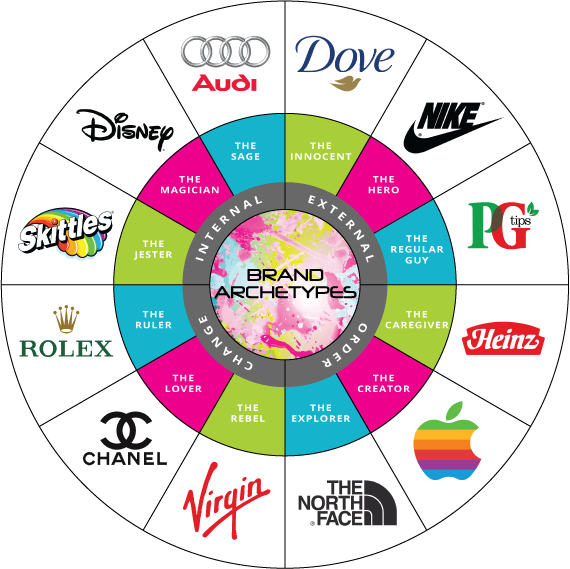
\includegraphics[width=0.49\linewidth]{img/brand_archetypes1} 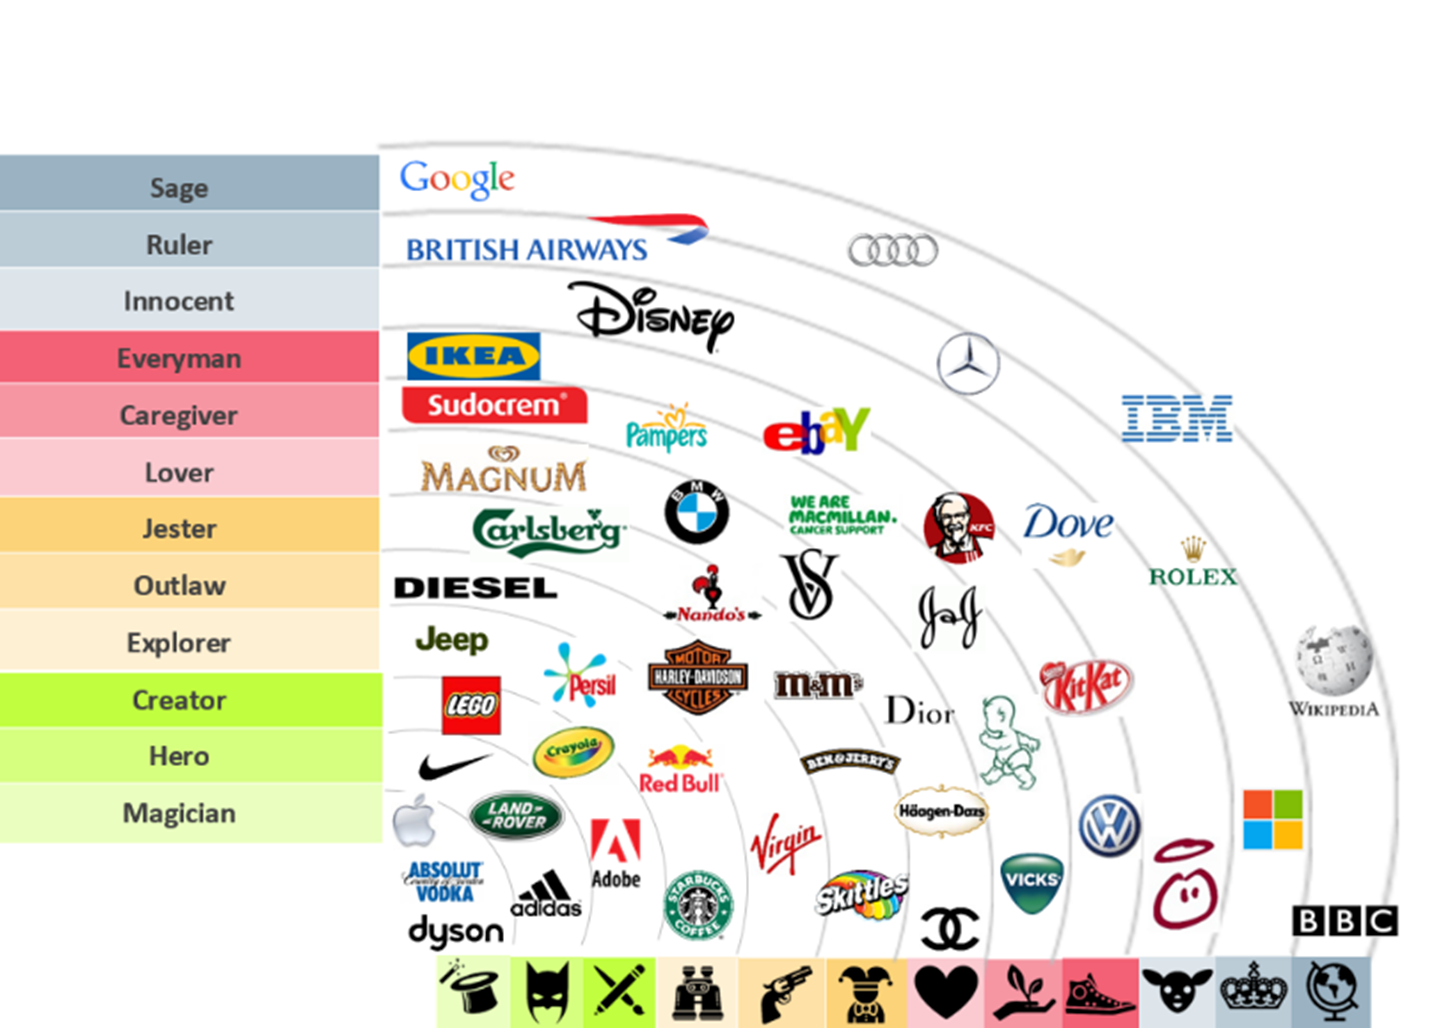
\includegraphics[width=0.49\linewidth]{img/brand_archetypes2} 

}

\caption{Examples of association between existing brands and archetypes (retrieved from 'https://visionone.co.uk/app/uploads/brand-archetype-wheel.png' and 'https://www.retailmarketing.com/wp-content/uploads/2017/09/Pic2.png').}\label{fig:unnamed-chunk-4}
\end{figure}

\hypertarget{recent-developpments}{%
\section{Recent Developpments}\label{recent-developpments}}

The coach Scott Jeffrey, after disguising random information as facts (``archetypes influence 99\% of human behavior''), ends up with a list of \href{https://scottjeffrey.com/archetypes-list/}{over 325} archetypes (!), suggesting that their number is even larger (``the reality is that there are thousands of archetypes. Each one possesses different behavioral patterns and subtleties''). Defining them as ``set pattern of behavior'', these fined-grained classifications are clearly different from archetypes as conceptualised in this book, i.e., as neuropsychological protostructures.

\hypertarget{a-scientific-archetypism}{%
\chapter{A Scientific Archetypism}\label{a-scientific-archetypism}}

\textbf{Warning: This is a work in progress, i.e., currently just a collection of unstructured information.}

Many archetype theorists have adopted a bottom-up approach, from Jung itself, exploring various cultures, myths, religions or the depths of Human's psyche (using tools of pseudo-access such as psychoanalysis or hypnosis). The archetypist's role was then to assemble and integrate the interpretations that emerged from these observations, in a theory that could be applied to explain these observations.

We will take the opposite approach. Based on scientific knowledge about evolution, biology and neuroscience, we will outline a plausible framework, that we will then test on observations.

One of the main angle of attacks could be the practical value of generic archetype. Yes, a loving mother and a fearless father are common tropes in Human existence. What is the point of creating a whole pseudo-theory around them? A collateral question would be, do they (as concepts) have any direct influence over our lives?

\hypertarget{the-main-archetypes}{%
\chapter{The Main Archetypes}\label{the-main-archetypes}}

\textbf{Warning: This is a work in progress, i.e., currently just a collection of unstructured information.}

The main archetypes discussed in this chapter reffered to as ``axial archetypes'', as they emerge from to the axes that structure our mental system. As this system grows and complexifies, its dimensionality increases, creating new planes and providing more coordinates to navigate in this space. As a result of the densification of this matrix, archetypes become more subtler, fine-grained and ultimately fading into the unicity that is characterising our identity.

Thus, archetypes are usually paired (as they are the two spaces created separated by a line), creating a symmetric and hierarchical structure. Importantly, they can be identified, and grouped, relative to their causing axis, which is often an important distinction that the organism has to learn in order to adapt.

Thus, evidence for archetypes can be indirectly gathered by demonstrating the existence and relevance of their axis of reference.

\hypertarget{masculine-and-feminine}{%
\section{Masculine and Feminine}\label{masculine-and-feminine}}

Existing theories and models often associate archetpyes with specific genders, namely ``feminine'' and ``masculine''. While this will also be the case in the current book, the reader must be aware that we see it mainly as a flexible (and convenient) appelation. In the archetypal framework, the Masculine and Feminine adjectives do not directly refer, nor are limited, to their respective biological genders, but rather to features of the two primordial archetypes, the father and the mother (see below). That does not preclude that a masculine archetype can be embodied by a female figure and \emph{vice versa}.

Moreover, another limitation of this pseudo-sexualised perspective is that it is, to some extent, anthropomorphic or primatomorphic (or at least mammalomorphic). Indeed, in these classes and families, males often endorse the role of protection, fighting for females through which reproduction can be achieved. However, other taxa of animals, with different reproduction systems, might have these roles changed, or reversed. For instance, in ants, the ruler and the warriors are Females, whereas the males are typically exhibiting roles that would be anthropomorphically labeled as feminine. Thus, while we will keep using Masculine and Feminine in their primatal sense, these adjectives may not be universally relevant.

\hypertarget{the-two-worlds}{%
\section{The Two Worlds}\label{the-two-worlds}}

The Outside \emph{vs.} the Inside, or the external and internal worlds (or Self vs.~non-Self), is the first axis differenciating our proto-experience.

Transcendal vs.~Natural.

The newborn is a fragile and dependent entity, which safety depends on the \emph{Mother} and the \emph{Father}. These are the first

Both are vectors of \textbf{protection}. The father protects from the outside world, unknown and dangerous, while the mother protects from internal dangers by fullfilling biological needs (hunger, thirst, affection, \ldots).

These two primordial archetypes will create the primordial axis, external vs.~internal worlds.

A secondary axis could be the real vs.~the unreal.

\begin{figure}

{\centering 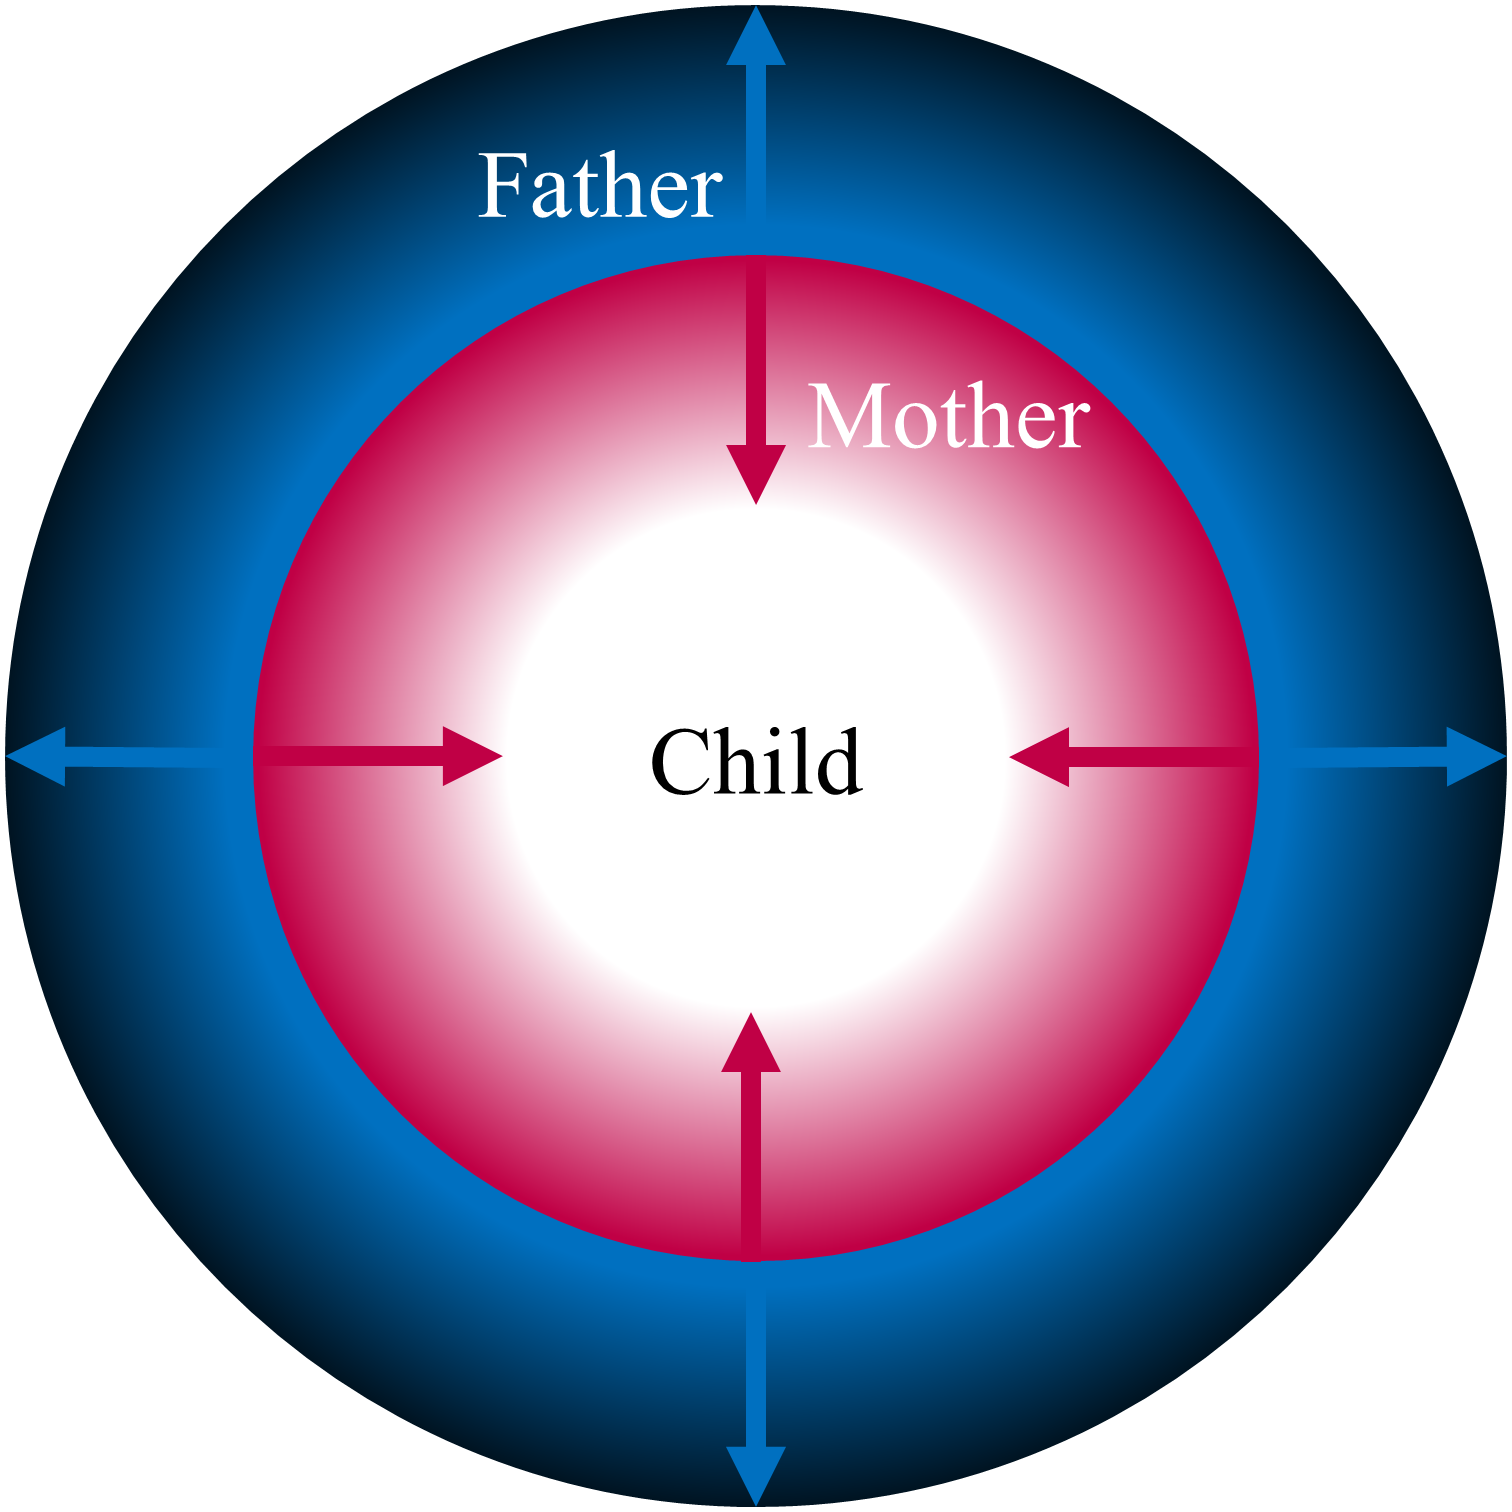
\includegraphics[width=\textwidth]{img/protection} 

}

\caption{The Primordial Axis.}\label{fig:unnamed-chunk-5}
\end{figure}

\hypertarget{known-vs.-unknown}{%
\section{\texorpdfstring{Known \emph{vs.} Unknown}{Known vs. Unknown}}\label{known-vs.-unknown}}

Knowledge

Knower of beyond vs.~knower of within.

The child wants to know, and understand this world around and within him. From the Mother, master of nature, stems out the \emph{Feminine Knower}. From the Father, master of the transcendent, stems out the \emph{Masculine Knower}.

\hypertarget{time}{%
\section{Time}\label{time}}

\hypertarget{moral}{%
\section{Moral}\label{moral}}

For elderly figures, this is assimilated with the place in the society, whether inside (priest, matron) or outside (hermit and witch). For young figures, this reflects the societal and cultural judgment. The hero and the virgin are pure archetypes of virtue, whereas the wanderer and the whore are usually societal and cultural outcasts.

\hypertarget{order}{%
\section{Order}\label{order}}

At one point, the realisation comes that all these figures are subordinated to an overarching ordering and structuring force, the \emph{Ruler}. Altough this archetype has often been related or embodied by Masculine entities, it does not need to be so, as it highly depends on societal and biologoical factors (related to the culture or Specie concerned). For instance, due to the cultural and political system of the western world (for instance, feodalism), the ruler position was generally connected to some level of physical protection offered (hence the king was usually glorified as a great warrior).

\hypertarget{death}{%
\section{Death}\label{death}}

Death is surely a major drive.

\hypertarget{the-artist}{%
\section{The artist}\label{the-artist}}

The artist is the integration of the feminine creation with the masculine transcendental nature of the object. Located at the centre, it shares aspects and potentialities of other archetypes. For instance, the artist can take uptake the purity, such as Michel-Angelo, or being the outcast, combining features of the hermit, living on the fringes of society, but also with the wanderer (as the rogue traveller and story-teller), as well as the whore () or the witch ().

\begin{figure}

{\centering 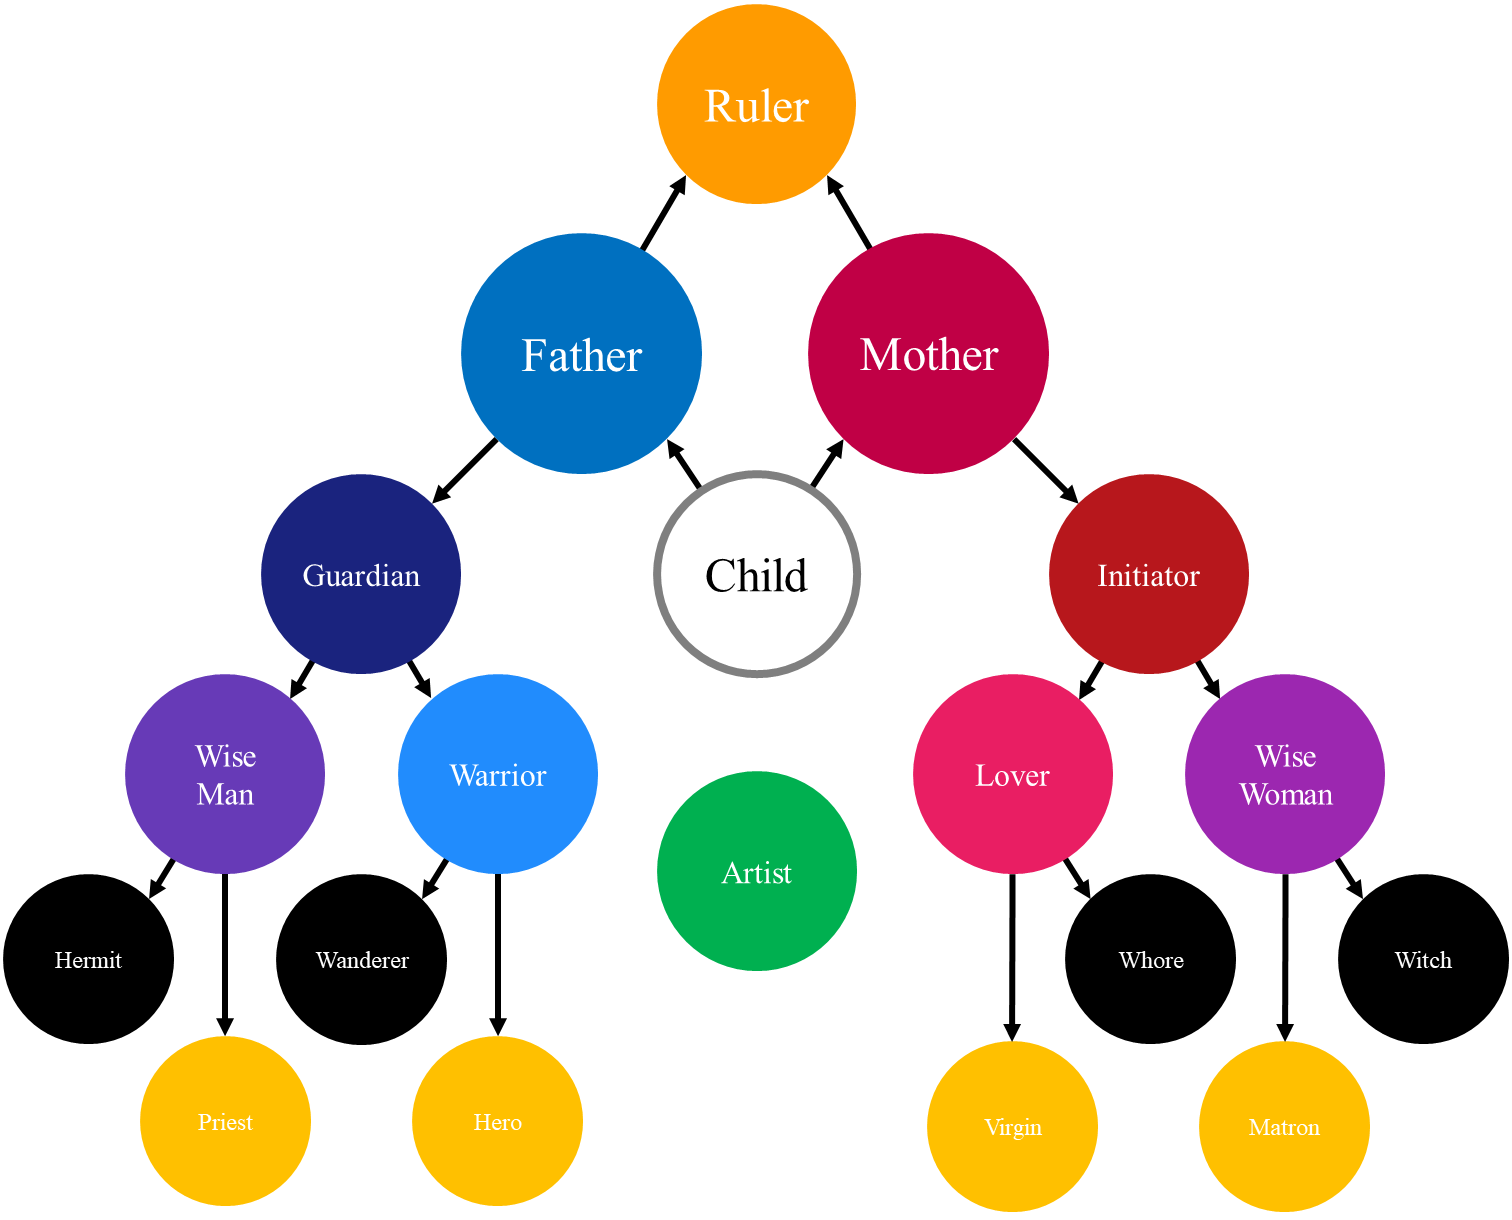
\includegraphics[width=\textwidth]{img/archetypes} 

}

\caption{The main archetypes and their hierarchical structure.}\label{fig:unnamed-chunk-6}
\end{figure}

\hypertarget{the-serpent}{%
\section{The Serpent}\label{the-serpent}}

The serpent represent the cyclical nature of existence. A mother creates a child, the child becomes the mother, and the cycle restarts.

Becoming an adult means facing the serpent. Alternative ways can be to embrace (becomeà the serpent (fulfilling the archetypes and becoming the Father or the Mother), or to battle the serpent, by trying to break the cycle.

\hypertarget{light-and-shadow}{%
\section{Light and Shadow}\label{light-and-shadow}}

The stronger the light, the darker the shadow.
Idea that everybody has a ``shadow'', a collection of morally reprehensible desires and thoughts, and that its strength is proportional to the amount of light shining from the persona. Yin and Yang. True peace of mind could be achieved by reuning them (The Grey Path).

\hypertarget{archetypes-and-psychology}{%
\chapter{Archetypes and Psychology}\label{archetypes-and-psychology}}

\textbf{Warning: This is a work in progress, i.e., currently just a collection of unstructured information.}

The archetypal framework developped in this book is by essence reductionist, exploring the abstract core features of cognition and essentializing them to concepts of pure abstraction. As such, archetypes do not directly relate to individual psychology, nor to anything tangible.

\hypertarget{archetypes-as-heuristics}{%
\section{Archetypes as Heuristics}\label{archetypes-as-heuristics}}

One could define an archetype is a basic frame facilitating a basic, instinctive, and intuitive understanding of a concept or a personality. This definition brings it close to a key concept in psychology, heuristics.

\hypertarget{relationship-with-personality}{%
\section{Relationship with Personality}\label{relationship-with-personality}}

\hypertarget{archetypes-and-the-brain}{%
\chapter{Archetypes and the Brain}\label{archetypes-and-the-brain}}

\textbf{Warning: This is a work in progress, i.e., currently just a collection of unstructured information.}

Do archetypes have a biological existence?

\hypertarget{origin}{%
\section{Origin}\label{origin}}

Are the archetypes innate? No, (altough they might have been favoured by evolution); they stem out of the redunduncies of existence.

\hypertarget{archetypes-as-neurocognitive-invariants}{%
\section{Archetypes as Neurocognitive Invariants}\label{archetypes-as-neurocognitive-invariants}}

contrary to Jung, these archetypes are not originating from some collective unconscious, but rather are created and maintained by the ontology of the individual, and patterns are crystilised out of the répétition and similarity accross individual ontologies (e.g., the presnece of a fatherly and a motherly figure, etc.)

\hypertarget{neurological-substrate}{%
\section{Neurological Substrate}\label{neurological-substrate}}

Attempts have been made to map archetypes unto brain structures \citep{samuels2003jung}. For instance, \citet{rossi1977cerebral} suggested that one could locate the archetypes in the right cerebral hemisphere, based on the idea that the left hemisphe would be primarily verbal and associational, and the right primarily visuospatial and apperceptive. In light of the current neuroscientific data, these theories appear as nonsensical and naive.

That being said, if archetypes are engrammed into the cognitive system, a biological basis has to exist. One potential answer is to reframe archetypism under the predictive coding framework. As such, archetypes could be seen as meta-priors.

\hypertarget{archetypal-stories}{%
\chapter{Archetypal stories}\label{archetypal-stories}}

\textbf{Warning: This is a work in progress, i.e., currently just a collection of unstructured information.}

Common motives in religions and myths beg the question of the existence or plausibility of archetypal stories.

\hypertarget{the-origin-of-religions}{%
\chapter{The Origin of Religions}\label{the-origin-of-religions}}

\textbf{Warning: This is a work in progress, i.e., currently just a collection of unstructured information.}

It is possible that archetypes have been deified, mother (nature and creation), father (protection and sky - the unreachable world).

Archetypes might have been integrated with a will to explain terryfing or unknown phenomena, such as storm, rain, fire, day-night cycle etc.

\bibliography{book.bib,packages.bib}


\end{document}
